\begin{frame}[fragile]{AlertDialog.Builder y Dialog con XML en Android}

\textbf{¿Qué es un Cuadro de Dialogo?} 
\begin{itemize} 
\item Es una ventana emergente que permite interactuar con el usuario. 
\end{itemize}

\textbf{¿Qué es AlertDialog.Builder?}
\begin{itemize}
    \item Clase utilizada para construir y mostrar diálogos emergentes.
    \item Permite definir título, mensaje, botones y eventos.
\end{itemize}


\textbf{Dialog con contenido XML:}
\begin{itemize}
    \item Permite usar una interfaz personalizada definida en un layout XML.
    \item Se establece su contenido en base al archivo XML.
\end{itemize}


\textbf{Ventajas del Dialogo Personalizado:}
\begin{itemize}
    \item Mayor personalización de la interfaz.
    \item Permite incluir EditText, imágenes, botones, etc.
\end{itemize}

\end{frame}



\begin{frame}[fragile]
\frametitle{Demo 11: Dialog y CustoDialog}
\begin{columns}
\column{0.80\linewidth}
Del Repositorio Github:
\begin{itemize}
\item Copiar el archivo \textit{MainActivity\_Demo11.java} (dentro del Folder códigosJAVA) al mismo directorio donde esta el MainActivity.java
\item Copiar el archivo \textit{activity\_main\_demo11.xml} (dentro del Folder Carpeta\_layout) al mismo directorio donde esta el activity\_main.xml
\item Copiar el archivo \textit{custom\_dialog.xml} (dentro del Folder Carpeta\_layout) al mismo directorio donde esta el activity\_main.xml.
\item Modificar en el archivo \textit{AndroidManifest.xml} la cadena \textit{.MainActivity\_Demo10} por \textit{.MainActivity\_Demo11}.
%\item Ir a la linea 22 de archivo del archivo \textit{MainActivity\_Demo09.java}, poner el cursos en la palabra (en Rojo) \textit{documentfile}, presionar la combinación ALT+ENTER, y seleccionar de la lista desplegable la opcion ``Add dependency on ....''. Esto quitará el error y hara los ajustes necesarios. 
\end{itemize}

%\begin{block}{Demo \#09}
%Un App que permite escribir el contenido de un EditText a un archivo y cargar el contenido de cualquier archivo en el EditText
%\end{block}


\column{0.20\linewidth}

\begin{center}
 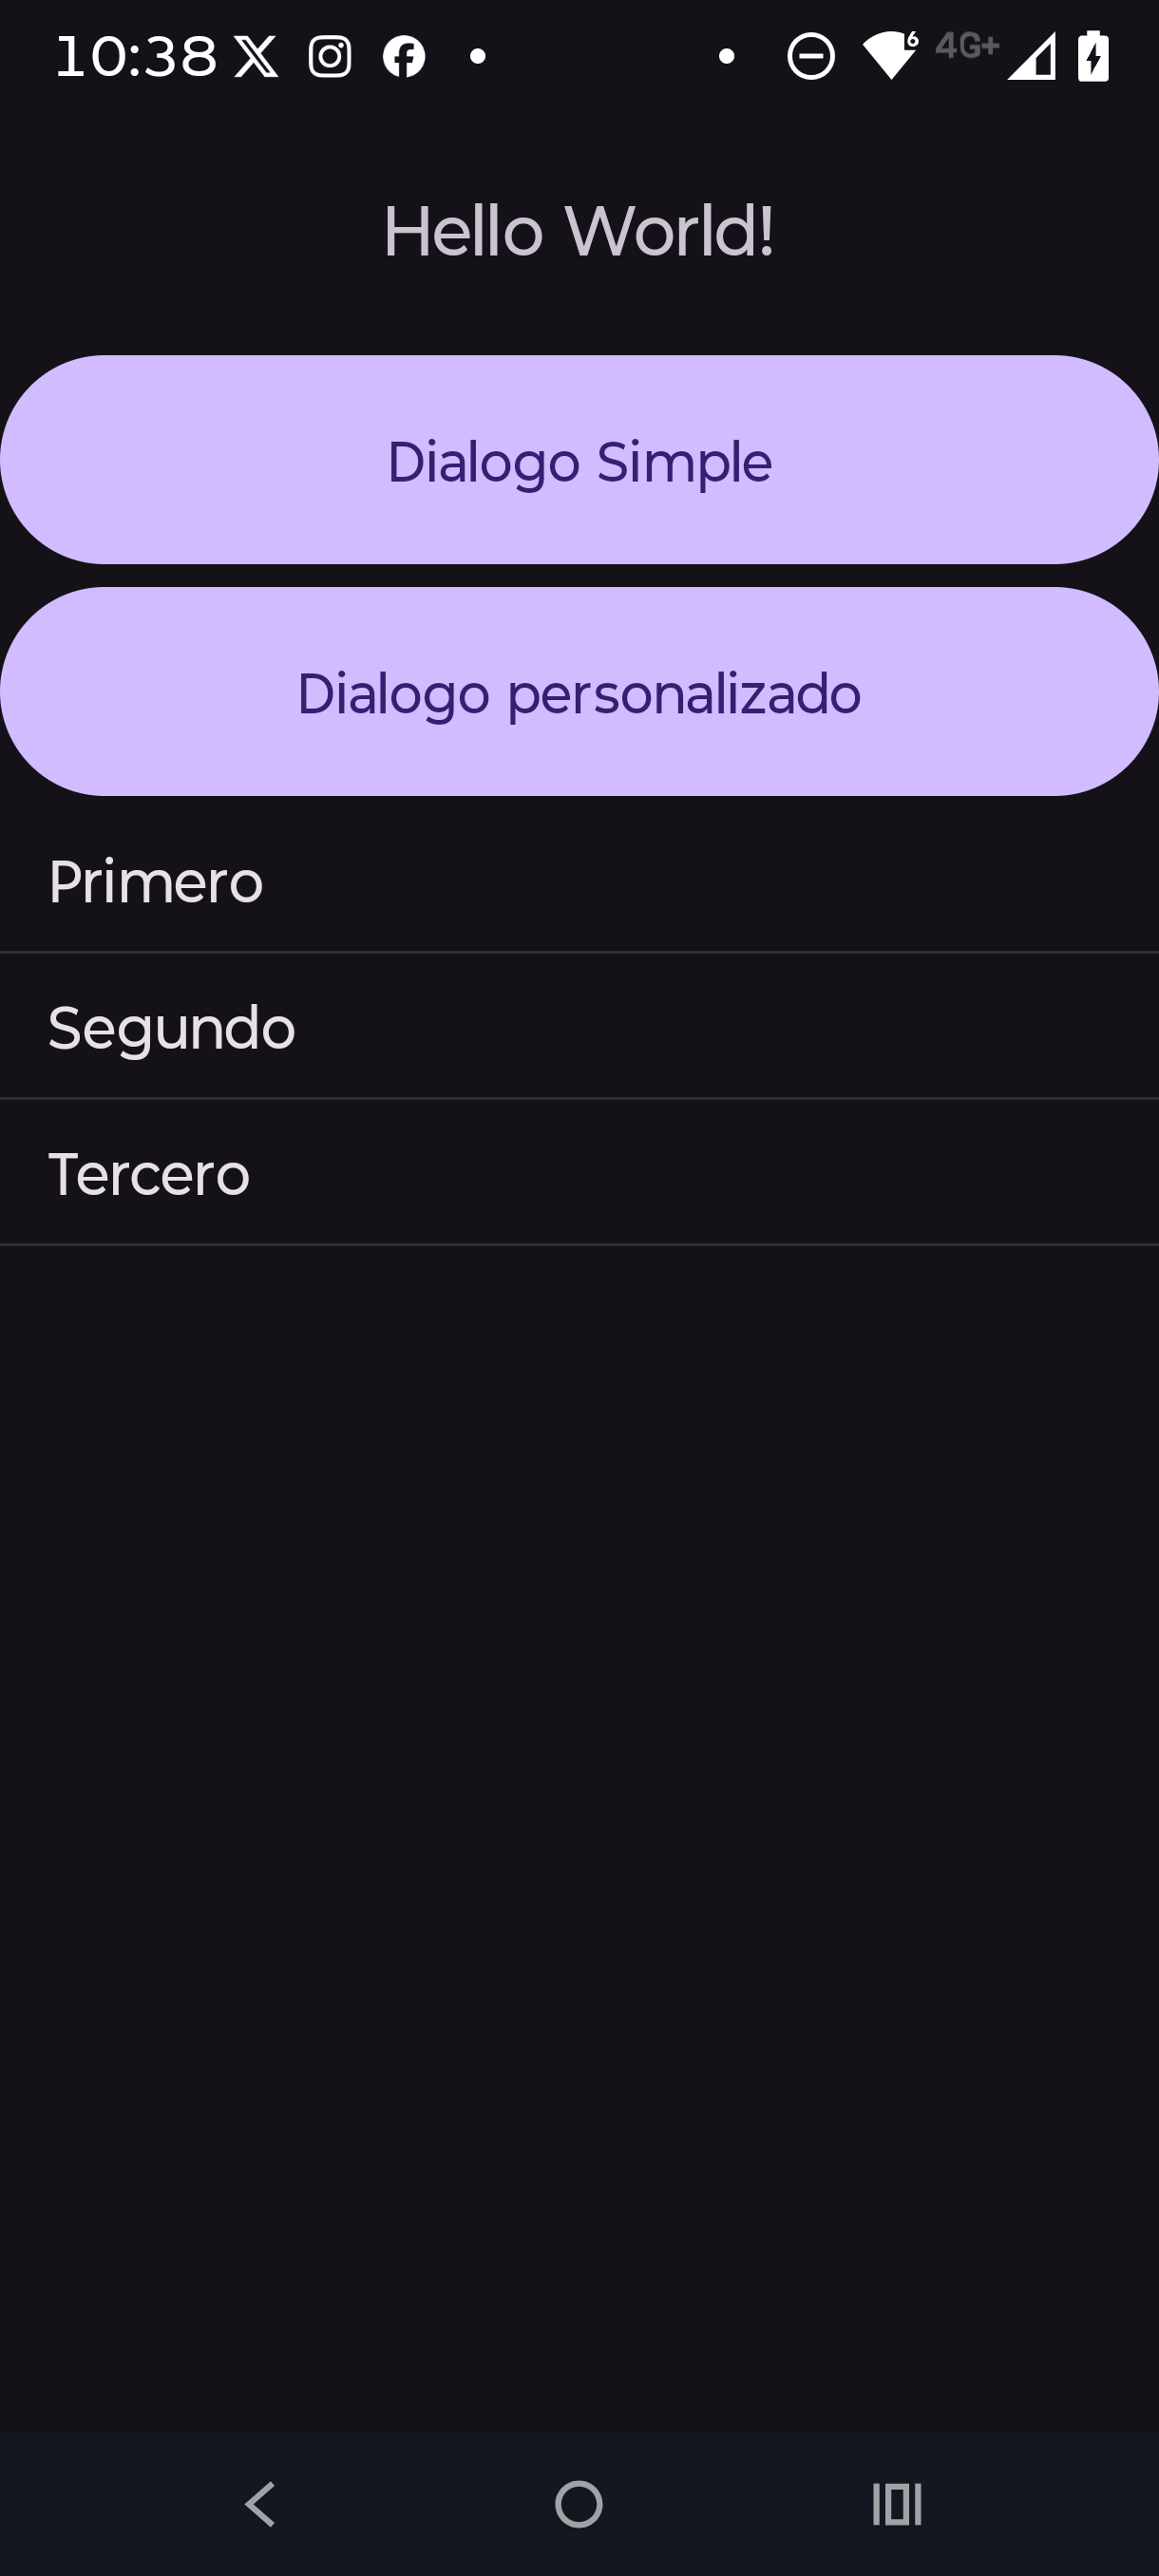
\includegraphics[width=0.98\textwidth]{02_TallerCBTis/figs/Demo11}
\end{center}

\end{columns}

\end{frame}

